\documentclass[12pt]{article}

\usepackage{amsmath}    % need for subequations
\usepackage{amssymb}
\usepackage{bussproofs}
\usepackage{verbatim}   % useful for program listings
\usepackage{color}      % use if color is used in text
\usepackage{subfigure}  % use for side-by-side figures
\usepackage{hyperref}   % use for hypertext links, including those to external documents and URLs
\usepackage[utf8]{inputenc}
\usepackage{ntheorem}
\usepackage{stmaryrd}
\usepackage{todonotes}
\usepackage{graphicx}

\theoremstyle{break}
\newcounter{counter}[subsection]

\newtheorem{definition}{Définition}[subsection]

\newtheorem{Theoreme}[definition]{Théorème}
\newtheorem{Corollaire}[definition]{Corollaire}
\newtheorem{prop}[definition]{Propriété}
\newtheorem{lemma}[definition]{Lemme}

\begin{document}
\begin{center}
{\large Extended README} \\ % \\ = new line
\end{center}
\section{Introduction}
Ce court document a pour but d'expliquer rapidement la structure de mon code sur ce sujet de stage et sa finalité.
L'objectif premier du stage était de réussir à formaliser sur Coq la décidabilité du critère de validité des preuves circulaires
dans $\mu$-MALL. 
Le code final que j'ai délivré a été très inspiré par trois travaux précédents:
\begin{itemize}
\item La bibliothèque YALLA d'Olivier Laurent consacrée à la logique linéaire.
\item Le code préliminaire produit par Xavier Onfroy sur la partie $\mu$-MALL de mon sujet.
\item La bibliothèque Natded-Master de Pierre Letouzey qui formalise la déduction naturelle en Coq.
\end{itemize}
La structure finale du code se décompose comme suit: 
\begin{center}
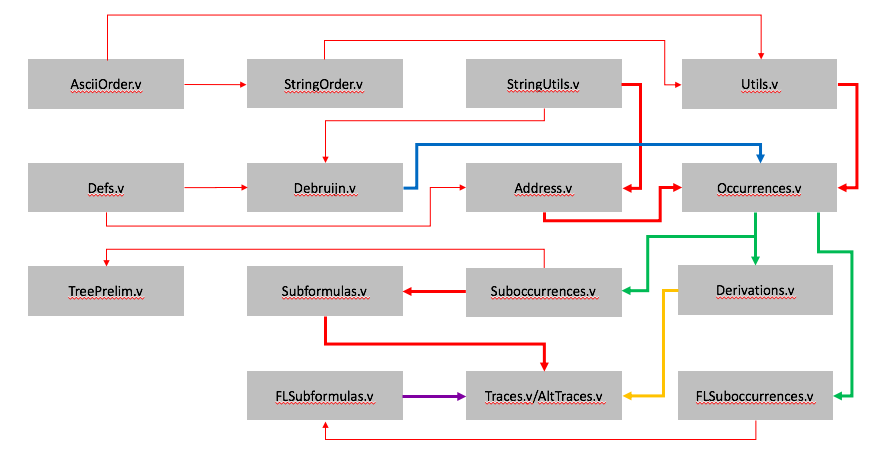
\includegraphics[scale=0.4]{/Links.png}
\end{center}
\begin{enumerate}
\item AsciiOrder.v, StringOrder.v, StringUtils.v et Utils.v fournissent des outils préliminaires pour les structure utilisées ultérieurement (listes, strings, etc.)
\item Defs.v introduit quelques notations et types de base
\item Debruijn.v définit les formules en utilisant les indices de Debruijn, ainsi qu'une multitude de fonctions et de lemmes sur ces dernières (substitution, etc.)
\item Address.v introduit les adresses d'occurrences et plusieurs résultats sur ces dernières (certains ne sont pas encore utilisés)
\item Occurrences.v unifie ces deux derniers fichiers en définissant les occurrences, puis introduit les séquents, les règles et les dérivations d'occurrences
\item Derivations.v introduit principalement la validité d'une dérivation (version booléenne et propriété inductive)
\item TreePrelim.v présente un travail préliminaire sur la structure d'arbre de formule, mais n'est pas encore utilisée dans la suite du développement
\item Suboccurrences.v définit la notion de sous-occurrence
\item Subformulas.v définit la notion de sous-formule "classique"
\item FLSuboccurrences.v définit très brèvement la notion de sous-occurrence, mais n'est pas encore utilisée
\item FLSubformulas.v introduit la notion de FL-sous-formules comme structure finie
\item Traces.v définit les traces et contient l'énoncé du critère de validité et de sa décidabilité 
\end{enumerate}

Dans la suite de ce document, je décrirai brièvement les fichiers clés du code, puis les pistes de poursuite du développement. 

\section{Debruijn.v}
On introduit ici d'abord les formules et le dual car on doit pouvoir parler de substitution par des formules. 
On définit la substitution, le niveau et la fermeture comme des classes de fonctions, qui sont ensuite définies successivement 
pour les formules, les séquents, les dérivations, etc.
Seule la substitution pour les variables est un peu spéciale car elle va de l'espace des variables dans celui des formules.
J'ai définit à la fin du fichier une propriété inductive qui caractérise le nombre de binders d'une formule car il m'a semblé qu'il pourrait être pertinent de 
raisonner par induction sur cette propriété, même si je ne m'en suis pas encore servi.
Les lemmes sur la substitution énoncés ici reserviront beaucoup lorsque l'on définira la substitution multiples dans FLSubformulas.v

\section{Address.v}
J'ai définit ici les adresses "à l'envers" par rapport à la structure classique, c'est-à-dire que le premier élément de l'addresse correspond à
la dernière direction empruntée dans la dérivation (vers la feuille).
La notion d'adresses disjointes sert ici seulement pour la règle de coupure. J'ai également inclus une fonction pour générer des adresses
fraîches vis-à-vis d'une liste d'addresse, en supposant qu'en prenant les addresses les plus longues dans une dérivation, on ne peut avoir à la fois
(i::a), (l::a) et (r::a) dans la dérivation (on ne peut pas utiliser une règle binaire et unaire en même temps).

\section{Occurrences.v}
La nouveauté dans ce fichier par rapport à Debruijn.v est l'introduction de la substitution d'occurrences, des règles logiques et des dérivations.
Plutôt que de définir les renommages comme des bijections d'ensembles d'adresses disjointes, qui sont des objets complexes, on définit la règle dite de
backedge. Pour ce faire, on associe à chaque dérivation une liste de séquents dits "backedgeables" (qu'on pourra enrichir au fur et à mesure qu'on 
remonte la dérivation) auxquels on associe un entier naturel qui désigne la distance entre le séquent actuel et le séquent du backedge considéré.
Par exemple, appliqué la règle (BackEdge 3) signifie que l'on fait un renommage du séquent actuel par le séquent présent trois règles en dessous.

\section{Derivations.v}
C'est dans ce fichier que l'on caractérise l'aspect le plus important des dérivatons, à savoir la validité d'application des règles qu'elles contiennent.
La version inductive de la validité est la plus lisible, et on s'arrêtera en particulier sur les critères suivants:
\begin{itemize}
\item Pour chaque application de règle, soit on conserve la même liste de séquents backedgeables en incrémentant leur distance, soit on 
	fait de même en rajoutant le séquent précédent comme backedge
\item Pour backedger vers un séquent dans cette liste (c'est une sorte de règle d'axiome), on demande seulement que le séquent actuel 
	ait les mêmes formules que le backedge considéré, dans le même ordre. 
\end{itemize} 
J'ai conservé la notion de prouvabilité d'un séquent introduit par Pierre Letouzey dans son code, mais ce n'est pas utilisé dans la suite.

\section{FLSubformulas.v}
On définit ici les FL-sous-formules comme une liste, par l'intermédiaire d'une liste de couple qui permet de mémoriser la définition de chaque
variable une fois celle-ci bindée. On définit donc cette liste de couple, quelques propriétés, et enfin la substitution multiple dans une formule 
(comme on ne substitue que des formules closes, cela ne pose pas de problème de capture).
J'ai également définit une fonction qui retourne cette liste de définition pour travailler sur des exemples.
FLSet permet de se débarasser des duplicatas dans la liste des FL-sous-formules.
Il est assez difficile d'énoncer des résultats sur cette structure de FL-sous-formule, car on est souvent bloqué par le cas d'une formule de point
fixe lors d'un raisonnement par induction, il est donc presque nécessaire de toujours définir les propriétés sur preFL F l en accompagnant le théorème
d'un invariant sur l.

\section{Traces.v}
Pour définir les traces, on passe d'abord par la notion de trace élémentaire, c'est-à-dire un seul parcours de l'arbre de dérivation de la racine
à l'une des feuilles, en suivant une formule. Cette notion a été définie relativement à un noeud de la dérivation, pour pouvoir énoncer la condition
de raccordement des traces élémentaires pour définir une trace.
On définit ensuite une trace comme une stream de trace élémentaires, avec quelques conditions supplémentaires de raccordement, à savoir que 
chaque trace élémentaire de la stream doit finir par un (BackEdge n), et que la trace élémntaire supplémentaire doit commencer au niveau du
séquent vers lequel on a backedgé.
Enfin, on énonce le critère de validité et sa décidabilité.

\section{AltTraces.v}
En raison de problème de manipulation des traces, ce fichier est une tentative d'introduction des streams comme fonction de n dans FTrace. L'énoncé
du critère est peu concluant car il requiert beaucoup de "il existe". Le fichier contient par ailleurs une définition fonctionnelle (Fixpoint) de la notion
de trace finie, peut-être plus manipulable pour prouver des théorèmes.

\section{Pistes à poursuivre}
J'énonce ici les points à éclaircir pour arriver à formaliser la décidabilité:
\begin{itemize}
\item Pour commencer, je n'ai travaillé ici que sur la partie logique. Xavier Onfroy avait également produit du code sur les $\omega$-automates, 
	il faudrait reprendre ce code et réussir à montrer l'équivalence entre le critère de validité que j'ai énoncé et l'inclusion des langages des
	deux automates énoncé dans la thèse d'Amina Doumane.
\item Par ailleurs, il faudrait enrichir la bibliothèque par davantage de lemmes et de propriétés, notammenent pour la notion de FL-sous-formules,
	qui est encore un peu compliquée à manipuler simplement.
\item Par ailleurs, il est nécessaire de creuser la partie relation d'ordre partielle de la FL-sous-formule, car elle est nécessaire à l'ensemble des
	lemmes et théorèmes d'existence de min sur les traces, etc. 
\item Enfin, la notion de traces étant CoInductive (stream), je n'ai pas énoncé de propriété dessus ni d'exemples car je ne sais pas manipuler les 
	cofixpoints, il est donc essentiel d'enrichir cette partie: existence du minimum dans une branche infinie, unicité, etc.
\end{itemize}

\end{document}